% Source: Lecture13.pdf, pages 1-8 (pages 9-10 are blank).
% Title on the source: "Lecture 13 - Other spin models".
\lecture{13}
\subsection{Generalized Ising models}
\subsubsection*{The anisotropic Ising model}

The spontaneous magnetization in the square-lattice Ising model (C.N.~Yang) is
\begin{equation}
  \bar M_{sp} = (1-\tilde k_<^2)^{1/8},\qquad\text{where}\quad \tilde k_< = \frac{1}{\tilde k_>} = \frac{1}{\sinh^2(2K)}.
\end{equation}
The free energy (and $\bar U$, $\bar C$, $\bar M_{sp}$) have also been calculated for other 2D lattices
and for the generalized case in which the spin--spin couplings are different in different lattice
directions, e.g.\ on the square lattice, for the ``anisotropic'' Ising model with
\begin{equation}
  \Ham = -\sum_{\mathbf r}\left(J_1\sigma_{\mathbf r}\sigma_{\mathbf r+\hat{\mathbf e}_1}
         + J_2\sigma_{\mathbf r}\sigma_{\mathbf r+\hat{\mathbf e}_2}\right),
\end{equation}
where $\hat{\mathbf e}_1 = \hat{\mathbf x}$ is a unit vector in the $x$ direction and
$\hat{\mathbf e}_2 = \hat{\mathbf y}$ is a unit vector in the $y$ direction. Define $K_1 = \beta J_1$
and $K_2 = \beta J_2$, $z_1 = e^{-2K_1}$, $z_2 = e^{-2K_2}$, $v_1 = \tanh K_1$, $v_2 = \tanh K_2$. Then
\begin{gather}
  f = \ln 2 + \frac{1}{2}\int_{-\pi}^{\pi}\frac{\dd^2\theta}{(2\pi)^2}\ln L,\nonumber\\
  L = \cosh(2K_1)\cosh(2K_2) - \sinh(2K_1)\cos\theta_1 - \sinh(2K_2)\cos\theta_2 .
\end{gather}
The critical temperature is defined by the condition
\begin{equation}
  \sinh(2K_1)\sinh(2K_2) = 1,\qquad\text{i.e.}\quad
  \sinh\left(\frac{2J_1}{\kB T_c}\right)\sinh\left(\frac{2J_2}{\kB T_c}\right) = 1 .
\end{equation}
This is the generalization of the condition $\sinh^2(2K) = 1$ in the isotropic ($J_1 = J_2$) case;
recall that for the isotropic case
\begin{equation}
  f = \ln 2 + \frac{1}{2}\int_{-\pi}^{\pi}\frac{\dd^2\theta}{(2\pi)^2}\ln\left[\cosh^2(2K)-\sinh(2K)(\cos\theta_1+\cos\theta_2)\right].
\end{equation}
For the FM case, the criticality condition gives a phase structure in the $K_1$--$K_2$ plane.

\begin{diagram}
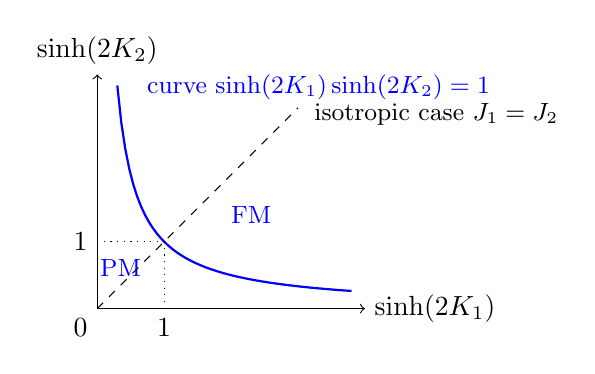
\begin{tikzpicture}[scale=0.85]
  \draw[->] (0,0) -- (4,0) node[right] {$\sinh(2K_1)$};
  \draw[->] (0,0) -- (0,3.5) node[above] {$\sinh(2K_2)$};
  \draw[thick,blue,domain=0.3:3.8,samples=60] plot (\x,{1/\x});
  \draw[dashed] (0,0) -- (3,3);
  \draw[dotted] (0,1) -- (1,1) -- (1,0);
  \node[below] at (1,0) {$1$}; \node[left] at (0,1) {$1$}; \node[below left] at (0,0) {$0$};
  \node[blue,font=\small] at (0.35,0.6) {PM};
  \node[blue,font=\small] at (2.3,1.4) {FM};
  \node[blue,anchor=west,font=\small] at (0.6,3.3) {curve $\sinh(2K_1)\sinh(2K_2) = 1$};
  \node[anchor=west,font=\small] at (3.1,2.9) {isotropic case $J_1 = J_2$};
\end{tikzpicture}
\diagramcaption{Phase structure of the anisotropic square-lattice Ising ferromagnet.}
\end{diagram}

Thus one can get FM LRO with a smaller $J_1$ and larger $J_2$ or vice versa, as well as the isotropic
case, $J_1 = J_2$. Here $\tilde k\to\tilde k_> = \sinh(2K_1)\sinh(2K_2)$, $\tilde k_< = (\tilde k_>)^{-1}$,
and $\bar M_{sp} = (1-\tilde k_<^2)^{1/8}$ as before. The critical behavior is the same as in the
isotropic case (provided that there is no frustration, e.g.\ for the FM case $J_i>0$ on all 2D lattices
and the AFM case on bipartite lattices).

There is a generalization of the FM and AFM ordering. E.g.\ on the square lattice as $T\to 0$, the LRO
is all $+$ or all $-$ for the FM, and the two checkerboard (N\'eel) patterns for the AFM. Now, again on
the square lattice, in addition to the FM case $\{J_1>0,J_2>0\}$ and the AFM case $\{J_1<0,J_2<0\}$,
there are the two mixed cases $\{J_1>0,J_2<0\}$ and $\{J_1<0,J_2>0\}$. These lead to a low-temperature
ordering as $T\to 0$ in which rows (for $J_1>0$, $J_2<0$) or columns (for $J_1<0$, $J_2>0$) alternate
in sign:
\begin{equation*}
  J_1>0,\ J_2<0:\quad
  \begin{array}{cccccc}
    - & - & - & - & - & -\\ + & + & + & + & + & +\\ - & - & - & - & - & -\\ + & + & + & + & + & +
  \end{array}
  \qquad\qquad
  J_1<0,\ J_2>0:\quad
  \begin{array}{cccccc}
    + & - & + & - & + & -\\ + & - & + & - & + & -\\ + & - & + & - & + & -\\ + & - & + & - & + & -
  \end{array}
\end{equation*}

\subsubsection*{Universality and additional couplings}

The fact that the critical behavior is the same for all of these cases (when there is no frustration)
is an example of the property that the critical behavior depends on the symmetry group of the
zero-field Hamiltonian (and the related space of the order parameter) and the dimensionality of the
lattice, but not on details of the lattice structure (2D: sq, tri, hc, \ldots; 3D: sc, bcc, fcc, hcp,
\ldots) or the spin--spin couplings (provided they are not $=0$ or $\infty$). Recall that $\Ham$ is
invariant under $\mathbb{Z}_2$ transformations (with group elements $\{1,-1\}$, where the $-1$ element
means $\sigma_i\to-\sigma_i\ \forall\,i$), independent of whether $J_1 = J_2$ or $J_1\ne J_2$, given zero
external field.

Thus, for example, this universality of the critical behavior means that the critical behavior is the
same if we add additional spin--spin couplings that respect the $\mathbb{Z}_2$ symmetry. For example,
in addition to the nearest-neighbor couplings, we could add next-nearest-neighbor couplings such as
\begin{align}
  \Ham = &-J_1\sum_{\mathbf r}\sigma_{\mathbf r}\sigma_{\mathbf r+\hat{\mathbf e}_1}
          - J_2\sum_{\mathbf r}\sigma_{\mathbf r}\sigma_{\mathbf r+\hat{\mathbf e}_2}\nonumber\\
         &- J_{\text{diag.}}\sum_{\mathbf r}\sigma_{\mathbf r}\sigma_{\mathbf r+\hat{\mathbf e}_1+\hat{\mathbf e}_2}
          &&\text{(e.g.\ }\sigma_{(0,0)}\sigma_{(1,1)})\nonumber\\
         &- J_{1,nnn}\sum_{\mathbf r}\sigma_{\mathbf r}\sigma_{\mathbf r+2\hat{\mathbf e}_1}
          &&\text{(e.g.\ }\sigma_{(0,0)}\sigma_{(2,0)})\nonumber\\
         &- J_{2,nnn}\sum_{\mathbf r}\sigma_{\mathbf r}\sigma_{\mathbf r+2\hat{\mathbf e}_2} + \cdots
          &&\text{(e.g.\ }\sigma_{(0,0)}\sigma_{(0,2)}).
\end{align}
These are all invariant under the $\mathbb{Z}_2$ symmetry of the $H = 0$ theory. Although one cannot
solve for $f(T,H=0)$ when these additional terms are present, they do not change the critical behavior
(assuming that they do not produce frustration). The approximation of keeping only nn spin--spin
couplings is usually a good one, although there are some materials where nnn spin--spin couplings are
non-negligible.

Note that in contrast, if one added an interaction term to $\Ham$ that violates the $\mathbb{Z}_2$
symmetry of the zero-field theory, such as a 3-spin coupling
$-J_{3sa}\sum_{\mathbf r}\sigma_{\mathbf r}\sigma_{\mathbf r+\hat{\mathbf e}_1}\sigma_{\mathbf r+\hat{\mathbf e}_2}$
(an ``L'' of three sites) or
$-J_{3sb}\sum_{\mathbf r}\sigma_{\mathbf r}\sigma_{\mathbf r+\hat{\mathbf e}_1}\sigma_{\mathbf r+2\hat{\mathbf e}_1}$
(three sites in a row), this \emph{does} change the critical behavior.

\subsubsection*{The spin-\texorpdfstring{$s$}{s} Ising model}

Another generalization of the Ising model is to have the spin variable $s_i$ take on more than 2 values,
in a way that retains the $\mathbb{Z}_2$ invariance, namely $s_i\in\{-s,-s+1,\ldots,s-1,s\}$. This is
called the ``spin-$s$ Ising model'' and is a natural classical model reflecting the property that a
quantum spin is a representation $s$ of $SU(2)$, with states
$\{|s,m_s\rangle\} = \{|s,-s\rangle,|s,-s+1\rangle,\ldots,|s,s-1\rangle,|s,s\rangle\}$, e.g.\
$s = 1/2$: $\{|1/2,-1/2\rangle,|1/2,1/2\rangle\}$; $s = 1$:
$\{|1,-1\rangle,|1,0\rangle,|1,1\rangle\}$, etc. With appropriate rescalings the spin-$1/2$ Ising
model then has $\sigma_i\in\{-1,1\}$, the spin-1 Ising model has $s_i\in\{-1,0,1\}$, etc., with
\begin{equation}
  \Ham = -J\sum_{e_{ij}}s_is_j,\qquad Z = \sum_{\{s_i\}}e^{-\beta\Ham}.
\end{equation}
Because this model has the same $\mathbb{Z}_2$ invariance, it has the same critical behavior. But it is
less studied because one has not been able to obtain an exact closed-form solution for $f$, $U$, $M$,
etc.\ even in the case of zero external magnetic field.

\subsection{The \texorpdfstring{$q$}{q}-state Potts model}

Another type of discrete spin model is the $q$-state Potts model. We have shown the equivalence of the
$q = 2$ Potts model and the (spin-$1/2$) Ising model. With zero-field
$\Ham = -J_P\sum_{e_{ij}}\delta_{\sigma_i\sigma_j}$, the symmetry group of the $q$-state Potts model is
the group of permutations of $q$ objects, $S_q$, of order $q!$. An example illustrates this invariance:
say $q = 3$. Then in the interaction of two adjacent spins, there are $q^2 = 9$ possible values of the
pair $\sigma_i\sigma_j$: the pairs $11$, $22$, $33$ with $\delta_{\sigma_i\sigma_j} = 1$, and the pairs
$12$, $21$, $13$, $31$, $23$, $32$ with $\delta_{\sigma_i\sigma_j} = 0$. Now transform all the spins
globally by one of the $q!$ elements of the permutation group $S_q$. Denote this element of $S_q$ by
$g$; $g(\sigma_i) = \sigma_i'$. For the cases where $\sigma_i = \sigma_j$, $g(\sigma_i) = g(\sigma_j)$, so
$\delta_{\sigma_i\sigma_j} = \delta_{g(\sigma_i)g(\sigma_j)} = 1$. By the definition of a group $G$, every
$g$ in $G$ has an inverse, $g^{-1}$, such that $gg^{-1} = g^{-1}g = 1$. If $\sigma_i\ne\sigma_j$, then
$g(\sigma_i)\ne g(\sigma_j)$, since if $g(\sigma_i) = g(\sigma_j)$, then
$g^{-1}g(\sigma_i) = \sigma_i = g^{-1}g(\sigma_j) = \sigma_j$, contradicting the assumption that
$\sigma_i\ne\sigma_j$. Since $\sigma_i\ne\sigma_j\Rightarrow g(\sigma_i)\ne g(\sigma_j)$,
$\delta_{\sigma_i\sigma_j} = \delta_{g(\sigma_i)g(\sigma_j)} = 0$. This proves that the zero-field Potts
$\Ham$ is invariant under $S_q$. Note that $S_2\approx\mathbb{Z}_2$. An external magnetic field term
$-H\sum_i\delta_{\sigma_i,1}$ breaks the $S_q$ symmetry explicitly and a spontaneous magnetization
$\ev{\sigma_i}$ breaks the $S_q$ symmetry spontaneously.

Recall the cluster formula (here $G$ means graph):
\begin{equation}
  Z(G,q,v_P) = \sum_{G'\subseteq G}q^{k(G')}v_P^{e(G')},
\end{equation}
where $G'$ = spanning subgraph of $G$, $v_P = e^{K_P}-1$ appearing in the identity
$e^{K_P\delta_{\sigma_i\sigma_j}} = 1 + v_P\delta_{\sigma_i\sigma_j}$, and $k(G')$ = \# of connected
components in $G'$, $e(G')$ = \# edges (= bonds) in $G'$. This cluster formula allows one to formally
generalize $q$ from a positive integer $q = 2,3,\ldots$ to a non-negative real number while keeping
$Z(G,q,v_P)>0$ (``Gibbs measure'') for FM $J_P>0$.

The $q$-state Potts ferromagnet has a continuous phase transition in 2D for $0<q\le 4$ ($Z = 0$ for
$q = 0$, but one can define $\tilde Z\equiv\lim_{q\to 0}(q^{-1}Z)$ to deal with the $q = 0$ case).

One commonly restricts to the integer cases $q = 2,3,4$, which have Hamiltonian representations. In
addition to the $q = 2$ (Ising) case, these provide interesting examples of critical behavior in 2D. In
contrast to the $q = 2$ Ising case, for $q\ne 2$, no closed-form expression has ever been calculated for
$f(T,H=0)$ (and obviously also not for $f(T,H\ne 0)$), but the critical exponents have been determined,
and they are rational, just as was true for the $q = 2$ case. For example, for the $q = 3$ Potts
ferromagnet in 2D, these exponents are
\begin{align*}
  q = 3:&\quad \alpha = \alpha' = \frac{1}{3},\enspace \beta = \frac{1}{9},\enspace \gamma = \gamma' = \frac{13}{9},
          \quad \nu = \nu' = \frac{5}{6},\enspace \delta = 14,\enspace \eta = \frac{4}{15},\\
  \text{vs. } q = 2:&\quad \alpha = \alpha' = 0\ \text{(log div.)},\enspace \beta = \frac{1}{8},\quad
          \gamma = \gamma' = \frac{7}{4},\enspace \nu = \nu' = 1,\enspace \delta = 15,\enspace \eta = \frac{1}{4} .
\end{align*}
The $q = 1$ Potts model, defined in the usual way, is trivial, since $\delta_{\sigma_i\sigma_j} = 1\ \forall\,i,j$,
so
\begin{equation}
  Z(\Lambda,q=1,v_P) = e^{K_Pe(\Lambda)} = e^{K_P(\Delta/2)n(\Lambda)},\qquad
  f = \lim_{n\to\infty}n^{-1}\ln Z = K_P\frac{\Delta}{2} .
\end{equation}

\subsubsection*{Landau--Ginzburg theory with a cubic term}

An interesting point concerns the Landau--Ginzburg formalism applied to the Potts model for $q\ne 2$,
e.g.\ $q = 3$. Because there is no $\mathbb{Z}_2$ invariance, the LG form of the Helmholtz free energy
$A(T,M)$ contains a cubic term:
\begin{equation}
  A(T,M) = L_0 + L_1M + L_2M^2 + L_3M^3 + L_4M^4 .
\end{equation}
As before, the $L_0$ term does not affect the determination of the minima of $A$, and the $L_1M$ term is
absent since otherwise $\left.\partial A/\partial M\right|_{M=0}\ne 0$, so $M = 0$ could not be a minimum of $A$ even at
high $T$. So
\begin{equation}
  A(T,M) = L_2M^2 + L_3M^3 + L_4M^4 .
\end{equation}
This can lead to a first-order transition.

\begin{diagram}
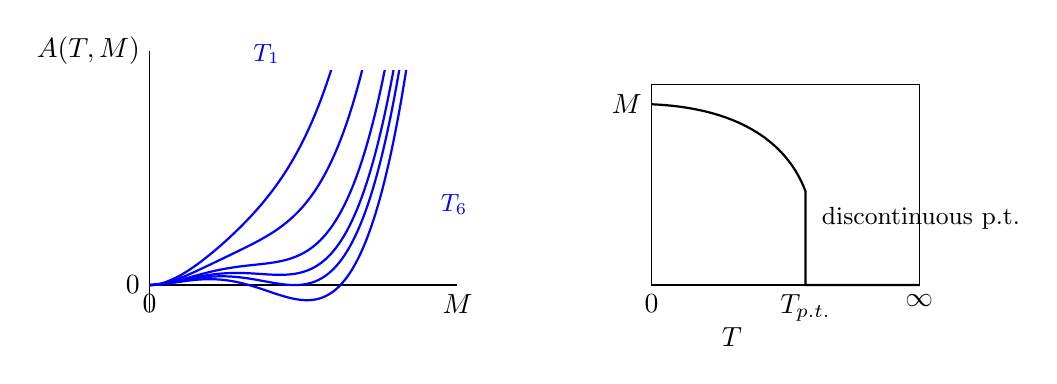
\begin{tikzpicture}[scale=0.85]
  \draw (0,-0.4) -- (0,3.5) node[left] {$A(T,M)$}; \draw (0,0) -- (4.6,0) node[below] {$M$};
  \begin{scope}
  \clip (0,-0.5) rectangle (4.5,3.2);
  \foreach \a in {1.6,1.25,1.0,0.9,0.833,0.75} {
    \draw[blue,thick,domain=0:3.4,samples=80,smooth] plot ({1.3*\x},{0.9*(\a*\x*\x - \x*\x*\x + 0.3*\x*\x*\x*\x)});
  }
  \end{scope}
  \node[blue,font=\small] at (1.75,3.45) {$T_1$};
  \node[blue,font=\small] at (4.55,1.2) {$T_6$};
  \node[left] at (0,0) {$0$}; \node[below] at (0,0) {$0$};
  \begin{scope}[xshift=7.5cm]
    \draw (0,0) rectangle (4,3);
    \draw[thick] (0,2.7) .. controls (1.2,2.65) and (2.0,2.2) .. (2.3,1.4) -- (2.3,0) -- (4,0);
    \node[below] at (0,0) {$0$}; \node[below] at (2.3,0) {$T_{p.t.}$}; \node[below] at (4,0) {$\infty$};
    \node[below=12pt] at (1.2,0) {$T$};
    \node[left] at (0,2.7) {$M$};
    \node[anchor=west,font=\small] at (2.4,1.0) {discontinuous p.t.};
  \end{scope}
\end{tikzpicture}
\diagramcaption{For $q\ne 2$: Landau--Ginzburg free energy with a cubic term, for
$T_1>T_2>\cdots>T_6$. As $T\searrow T_5$, the minimum of $A$ jumps discontinuously from the
$S_3$-symmetric value $M = 0$ to a nonzero value.}
\end{diagram}

It turns out that the phase transition between the $S_q$-symmetric high-temperature phase and the
low-temperature phase with spontaneous breaking of the $S_q$ symmetry and ferromagnetic LRO is
first-order for the $q$-state Potts model with $q\ne 2$ in $d = 3$, and in $d = 2$ for $q>4$, while for
$0\le q\le 4$, it is continuous. (The $q = 1$ case is trivial when defined by setting $q = 1$ before
taking the thermodynamic limit, but this does not commute with the opposite order of limits, i.e.\ the
thermodynamic limit first, with $q\in\mathbb{R}$, $q\ne 1$, and then letting $q\to 1$.)

\subsection{Continuous-spin models}
\subsubsection*{The Mermin--Wagner theorem}

Now proceed to continuous-spin models, e.g.\ $O(N)$ spin models with
\begin{equation}
  \Ham = -J\sum_{e_{ij}}\mathbf{S}_i\cdot\mathbf{S}_j - \mathbf{H}\cdot\sum_i\mathbf{S}_i,\qquad
  \mathbf{S}_i\in S^{N-1},\qquad
  Z = \int\left[\prod_i\dd\mathbf{S}_i\right]e^{-\beta\Ham},
\end{equation}
with $\mathbf{S}_i = (S_{1i},S_{2i},\ldots,S_{Ni})$, $|\mathbf{S}_i| = 1$, e.g.\ for $N = 2$,
$\mathbf{S}_i = (S_{1i},S_{2i}) = (\cos\theta_i,\sin\theta_i)$.

Recall a basic difference in the LG Helmholtz energy as a function of $M$ in the $\mathbb{Z}_2$ Ising
case (formally, $N = 1$ $O(N)$) and $O(N)$, $N\ge 2$. Illustrate this for $O(2)$:
$\mathbf{M} = \ev{\mathbf{S}} = \ev{(S_1,S_2)}$, with $M = |\mathbf{M}|$, $M_1 = \ev{S_1}$,
$M_2 = \ev{S_2}$.

\begin{diagram}
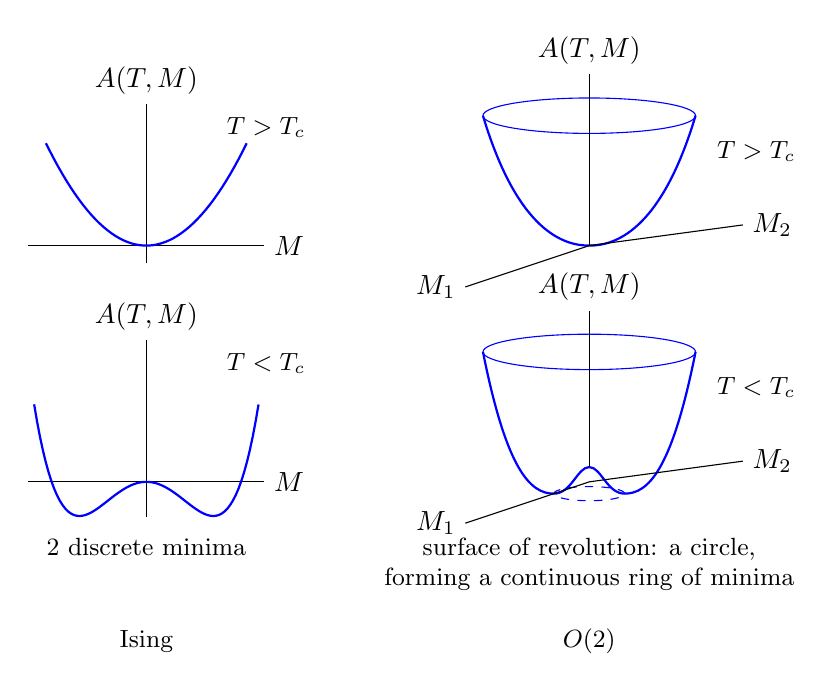
\begin{tikzpicture}[scale=0.75]
  \draw (-2,0) -- (2,0) node[right] {$M$}; \draw (0,-0.3) -- (0,2.4) node[above] {$A(T,M)$};
  \draw[thick,blue,domain=-1.7:1.7,samples=50] plot (\x,{0.6*\x*\x});
  \node[font=\small,anchor=west] at (1.2,2.0) {$T>T_c$};
  \begin{scope}[yshift=-4cm]
  \draw (-2,0) -- (2,0) node[right] {$M$}; \draw (0,-0.6) -- (0,2.4) node[above] {$A(T,M)$};
  \draw[thick,blue,domain=-1.9:1.9,samples=80] plot (\x,{-0.9*\x*\x+0.35*\x*\x*\x*\x});
  \node[font=\small,anchor=west] at (1.2,2.0) {$T<T_c$};
  \node[font=\small] at (0,-1.1) {2 discrete minima};
  \end{scope}
  \node[font=\small] at (0,-6.7) {Ising};
  \begin{scope}[xshift=7.5cm]
    \draw[thick,blue] (-1.8,2.2) .. controls (-1.2,0.2) and (-0.4,0) .. (0,0) .. controls (0.4,0) and (1.2,0.2) .. (1.8,2.2);
    \draw[blue] (0,2.2) ellipse (1.8 and 0.3);
    \draw (0,0) -- (0,2.9) node[above] {$A(T,M)$};
    \draw (0,0) -- (2.6,0.35) node[right] {$M_2$}; \draw (0,0) -- (-2.1,-0.7) node[left] {$M_1$};
    \node[font=\small,anchor=west] at (2.0,1.6) {$T>T_c$};
    \begin{scope}[yshift=-4cm]
      \draw[thick,blue] (-1.8,2.2) .. controls (-1.4,0.2) and (-1.0,-0.2) .. (-0.6,-0.2) .. controls (-0.3,-0.2) and (-0.2,0.25) .. (0,0.25)
            .. controls (0.2,0.25) and (0.3,-0.2) .. (0.6,-0.2) .. controls (1.0,-0.2) and (1.4,0.2) .. (1.8,2.2);
      \draw[blue] (0,2.2) ellipse (1.8 and 0.3);
      \draw[blue,dashed] (0,-0.2) ellipse (0.6 and 0.12);
      \draw (0,0.25) -- (0,2.9) node[above] {$A(T,M)$};
      \draw (0,0) -- (2.6,0.35) node[right] {$M_2$}; \draw (0,0) -- (-2.1,-0.7) node[left] {$M_1$};
      \node[font=\small,anchor=west] at (2.0,1.6) {$T<T_c$};
      \node[font=\small,align=center] at (0,-1.4) {surface of revolution: a circle,\\ forming a continuous ring of minima};
    \end{scope}
    \node[font=\small] at (0,-6.7) {$O(2)$};
  \end{scope}
\end{tikzpicture}
\diagramcaption{The Landau--Ginzburg free energy for the Ising and $O(2)$ models. (In the extension
to quantum field theory, the $m^2$ of a particle is the curvature of $V$,
$\partial^2V/\partial\phi^2|_{\min}$. N.B.: in the $O(2)$ case, this is 0 going around the ring of
degenerate minima.)}
\end{diagram}

This difference reflects the fact that the magnetization in the Ising model can only take on 2 values,
$M = \pm M_0$, but in the $O(2)$ model the vector spin can take on a continuous infinity of values,
$\mathbf{M} = (\cos\theta_0,\sin\theta_0)$ where $-\pi<\theta_0\le\pi$. To disorder incipient order in
the Ising model requires a discrete energy difference (flipping one spin in a sea of $+$ spins costs
$\Delta U = 2J\Delta = 8J$), whereas in contrast, to disorder an incipient ordered state in the $O(2)$
(in general, $O(N)$ with $N\ge 2$) model requires an arbitrarily small energy increment,
$\uparrow\uparrow\uparrow\uparrow\ \to\ \uparrow\uparrow\nearrow\nearrow$ etc. This is related to the
connected continuous $\infty$ of $\mathbf{M}$ values, all of which minimize $A(T,|\mathbf{M}|)$ at
$T<T_c$: the circular ring of minima for the $O(2)$ model shown in the graph.

This ease of disordering an incipient ordered state has the effect that a spin system at finite
temperature that is invariant under a continuous global symmetry group $G$ does not exhibit a phase
transition with spontaneous symmetry breaking (SSB) of this symmetry in $d = 2$ dimensions
(\emph{Mermin--Wagner Theorem}). This is connected with the Nambu--Goldstone Theorem, namely that
spontaneously breaking a continuous global symmetry leads to massless modes. In particle physics
(quantum field theory) these are massless elementary particles. In statistical mechanics, they are
modes disordering incipient order. In the illustrative $O(2)$ model, they can be seen as a consequence
of the continuous degeneracy of the minima of the energy: the circular ring of minima in the plot of
the free energy $A(T,M)$.

The case $T = 0$ is special, because here the minimization of the free energy reduces to the
minimization of the internal energy $U$, which is minimized for $M\ne 0$, i.e.\ nonzero spontaneous
magnetization (assuming no frustration).

This theorem does allow a system with a continuous symmetry group $G$ to have a finite-temperature phase
transition, as long as this does not spontaneously break the symmetry $G$, i.e.\ in a spin model, as
long as the spontaneous magnetization is zero.

\subsubsection*{The Kosterlitz--Thouless transition}

An example is the 2D $O(2)$ model with
\begin{equation}
  \Ham = -J\sum_{e_{ij}}\mathbf{S}_i\cdot\mathbf{S}_j,\qquad \mathbf{S}_i = (\cos\theta_i,\sin\theta_i).
\end{equation}
The 2D $O(2)$ model has a phase transition that involves dissociation of vortex pairs (``molecules'').
Recall that the vortices arise because the homotopy group $\pi_1(S^1)$ is nontrivial:
$\pi_1(S^1) = \mathbb{Z}$, where $\pi_1(G)$ is the set of continuous maps of $S^1\to G$. Now
$O(2)\sim U(1)\sim S^1$; spins ``live'' in $S^1$, the circle.

\begin{diagram}
\begin{tikzpicture}[scale=0.6,>=Stealth]
  \foreach \r in {0.7,1.3} \foreach \a in {0,45,...,315}
    \draw[->] ({\r*cos(\a)},{\r*sin(\a)}) -- ++({\a+90}:0.45);
  \node[font=\small,align=center] at (0,-2.6) {$n = 1$ element\\ of $\pi_1(S^1)$\\ (denote as v)};
  \begin{scope}[xshift=5cm]
  \foreach \r in {0.7,1.3} \foreach \a in {0,45,...,315}
    \draw[->] ({\r*cos(\a)},{\r*sin(\a)}) -- ++({-\a+90}:0.45);
  \node[font=\small,align=center] at (0,-2.6) {$n = -1$ element\\ of $\pi_1(S^1)$, opposite\\ vorticity (denote as $-$v)};
  \end{scope}
  \begin{scope}[xshift=10.5cm]
    \draw (0,0) ellipse (1.5 and 0.8); \node at (-0.6,0) {v}; \node at (0.6,0) {$-$v};
    \draw[->,blue] (1.8,0) -- (2.8,0);
    \node[blue,font=\small] at (2.3,1.1) {as $T\nearrow T_c$};
    \draw (3.6,0) circle (0.5); \node at (3.6,0) {v};
    \draw (5.0,0) circle (0.5); \node at (5.0,0) {$-$v};
    \node[font=\small,align=center] at (2.5,-2.6) {``topological\\ defect-driven p.t.''};
  \end{scope}
\end{tikzpicture}
\diagramcaption{Vortex configurations. At low $T$, the vortices are bound in vortex--antivortex pairs;
as $T\nearrow T_c$ the pairs dissociate.}
\end{diagram}

There is no magnetization in the low-temperature phase, and this phase transition does \emph{not} break
the $O(2)$ invariance. This was studied by Kosterlitz and Thouless, also Berezinskii, and is known as
the KT or BKT phase transition in the 2D $O(2)$ model. Monte Carlo simulations have confirmed the
picture of unbinding of vortex--antivortex pairs as $T\nearrow T_c$.

For $O(N)$ spin models with $N\ge 3$ in 2d, studies indicate no phase transition at finite temperature.
